% =============================================================================
% Pillar 3 — measured scale-up: unsaturated iso-compute sweep (Colab L4) and
% Qwen3-8B/GSM8K pass@k of adapters trained at four group sizes.
% Drivers: platform_colab/p3_isocompute_groupsize.py (training),
%          platform_colab/p3_isocompute_analyze.py (tables, figure)
% Inputs:  experiments/results/p3_isocompute/*.json (40 runs)
%          experiments/results/w2_groupsize_passk_wandb_export.tsv
%          experiments/tinker-runs/results/campaign_v2_20260419_111623.json
% =============================================================================
\section{Group Size Off the Ceiling: Measured Iso-Compute Sweeps}
\label{sec:group-size-scaleup}

The sweep of Section~\ref{sec:group-size} is saturated and holds the step count
fixed, so larger $G$ also gets more rollouts. This section removes both
limitations: it fixes the number of generated rollouts per step for every $G$,
uses a task the base model mostly fails, and adds $G{=}32$ and unwhitened control
arms.

\paragraph{Protocol.}
Same minimal GRPO as Section~\ref{sec:group-size} (Qwen2.5-0.5B, LoRA rank $16$ on
$q$/$v$, Adam $10^{-4}$, temperature $1.0$, sequence-mean log-probability, no KL or
clipping, one update per batch), with three changes
(\texttt{platform\_colab/p3\_isocompute\_groupsize.py}, one NVIDIA L4 per run):
(i) \emph{iso-compute}: every step generates $128$ completions, i.e.\ $128/G$
prompts with $G$ completions each, so all arms use the same rollouts and the same
$60$ optimizer steps; (ii) an \emph{unsaturated task}: two-digit multiplication
($a\times b$, $a,b\in\{10,\dots,99\}$, at most $12$ new tokens), on which the base
model scores $0.198$ greedy on $400$ held-out problems (mean over seeds) (two-operand addition: $0.945$);
(iii) \emph{whitening control}: in addition to GRPO's
$\hat A_i=(r_i-\bar r)/(\sigma_r+10^{-6})$, arms with $A_i=r_i-\bar r$ (no $1/\sigma_r$).
Whitened arms use seeds $\{42,123,456,789,1024\}$, unwhitened arms
$\{42,123,456\}$; each seed fixes a held-out set of $400$ problems shared by all arms
with that seed (training prompts are drawn fresh every step).

\paragraph{Held-out accuracy does not improve with $G$ at equal compute.}
Table~\ref{tab:groupsize-isocompute} and Figure~\ref{fig:groupsize-isocompute}
report the results. Every arm learns: held-out accuracy rises from $0.198$ to
$0.58$--$0.61$. Across $G\in\{2,4,8,16,32\}$ the whitened means are $0.598$,
$0.612$, $0.599$, $0.597$ and $0.580$. The largest difference, $G{=}4$ minus
$G{=}32$, is $+0.032$ (Welch $p{=}0.032$ at $n{=}5$ per arm; $p{=}0.13$ after
Bonferroni correction over the four comparisons with the best arm); all other
contrasts have $p>0.3$. At equal rollouts, larger groups therefore did not buy
held-out accuracy on this task, and $G{=}32$ was, if anything, slightly worse.
Last-10 training reward rises mildly with $G$ ($0.569\to0.590$), a training-set
effect that did not transfer to held-out problems.

\paragraph{ZVF falls with $G$, far above the homogeneous closed form.}
Mean ZVF falls from $0.826$ at $G{=}2$ to $0.353$ at $G{=}32$, so at $G{=}32$ almost
two-thirds of groups carry contrast versus under one-fifth at $G{=}2$. The
homogeneous closed form evaluated at each step's batch pass rate predicts much less
ZVF ($0.557\to0.049$): on this task most prompts are either almost always solved or
almost never, so batch-mean pass rates badly understate degenerate groups---the
heterogeneity effect of Section~\ref{sec:group-size}, here an order of magnitude
larger. Lowering ZVF by a factor of $2.3$ did not change held-out accuracy, so on
this evidence ZVF reduction is not, by itself, a lever on generalisation at
fixed compute.

\paragraph{Whitening has no measurable effect.}
On the three shared seeds, whitened minus unwhitened held-out accuracy is $+0.001$,
$-0.003$, $-0.002$, $+0.007$ and $+0.026$ for $G{=}2,\dots,32$ (paired $p\ge0.26$),
and the two variants have the same ZVF curve. The $1/\sigma_r$ factor rescales
non-degenerate groups but does not change which groups are degenerate, which is
consistent with the identical ZVF; its effect on accuracy is below what $n{=}3$
can detect.

\begin{table}[htbp]
\centering
\small
\resizebox{\linewidth}{!}{%
\begin{tabular}{cccccccc}
\toprule
Whitened & $G$ & Prompts/step & $n$ & Held-out acc.\ (95\% CI) & Gain vs base & Last-10 reward & ZVF (measured / closed form) \\
\midrule
yes & 2  & 64 & 5 & $0.598 \pm 0.032$ & $+0.400$ & 0.569 & 0.826 / 0.557 \\
yes & 4  & 32 & 5 & $0.612 \pm 0.029$ & $+0.414$ & 0.552 & 0.689 / 0.223 \\
yes & 8  & 16 & 5 & $0.599 \pm 0.034$ & $+0.401$ & 0.554 & 0.553 / 0.072 \\
yes & 16 & 8  & 5 & $0.597 \pm 0.026$ & $+0.400$ & 0.576 & 0.432 / 0.040 \\
yes & 32 & 4  & 5 & $0.580 \pm 0.015$ & $+0.382$ & 0.590 & 0.353 / 0.049 \\
\midrule
no  & 2  & 64 & 3 & $0.595 \pm 0.056$ & $+0.397$ & 0.570 & 0.828 / 0.547 \\
no  & 4  & 32 & 3 & $0.600 \pm 0.049$ & $+0.402$ & 0.546 & 0.690 / 0.215 \\
no  & 8  & 16 & 3 & $0.590 \pm 0.065$ & $+0.392$ & 0.560 & 0.562 / 0.064 \\
no  & 16 & 8  & 3 & $0.583 \pm 0.043$ & $+0.384$ & 0.562 & 0.442 / 0.041 \\
no  & 32 & 4  & 3 & $0.547 \pm 0.085$ & $+0.349$ & 0.581 & 0.357 / 0.044 \\
\bottomrule
\end{tabular}%
}
\caption{Iso-compute group-size sweep, Qwen2.5-0.5B / two-digit multiplication,
$128$ completions and one update per step, $60$ steps. Held-out accuracy is greedy
on $400$ seed-specific problems (base model $0.198$); intervals are $t$-based 95\%
CIs over seeds. ZVF is the mean over training; the closed form is
$p_t^G+(1-p_t)^G$ at each step's batch pass rate. Source:
\texttt{experiments/results/p3\_isocompute\_summary.tsv}.}
\label{tab:groupsize-isocompute}
\end{table}

\begin{figure}[htbp]
\centering
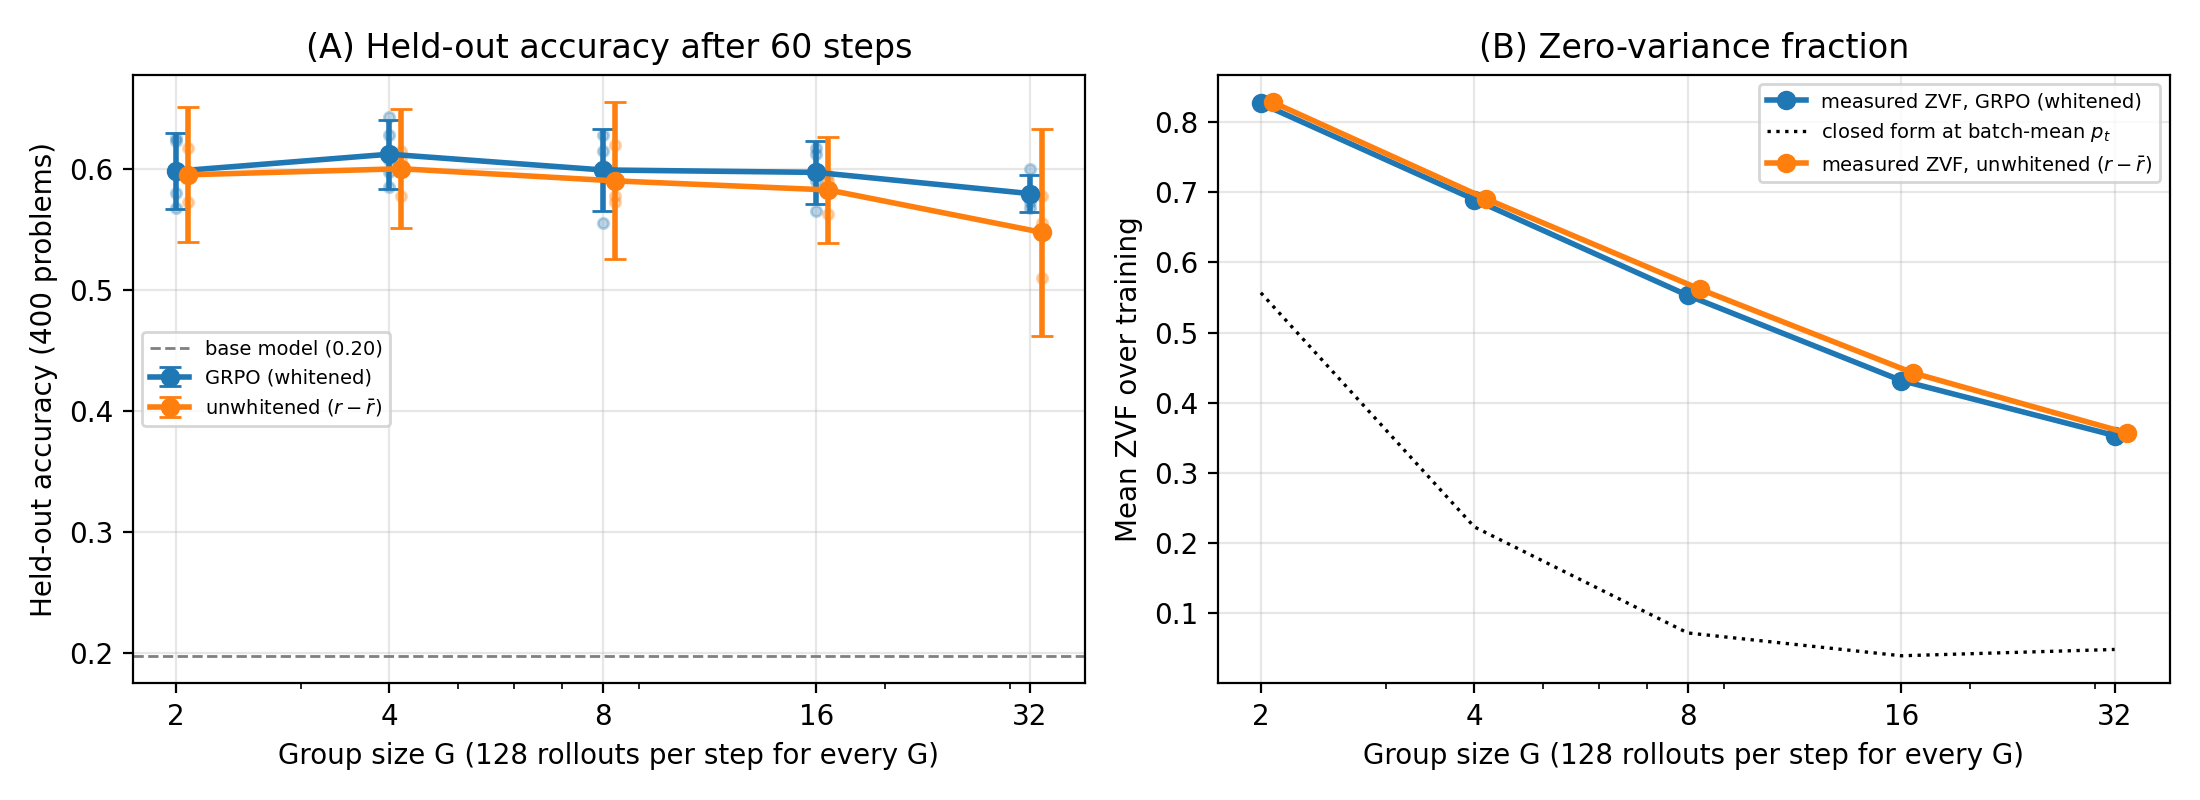
\includegraphics[width=\linewidth]{figures/group_size_isocompute_mul2.png}
\caption{\textbf{Iso-compute group-size sweep on an unsaturated task.}
\emph{(A)} Held-out accuracy after $60$ steps (points are seeds, bars are 95\% CIs)
for whitened GRPO and the unwhitened control; the dashed line is the base model.
\emph{(B)} Mean ZVF over training, with the homogeneous closed form at the batch
pass rate. Source: \texttt{platform\_colab/p3\_isocompute\_analyze.py}.}
\label{fig:groupsize-isocompute}
\end{figure}

\paragraph{Qwen3-8B on GSM8K: four group sizes, one training seed each.}
Separately, four Qwen3-8B LoRA adapters were trained with Tinker GRPO on GSM8K for
$30$ steps at learning rate $10^{-5}$ with $G\in\{2,4,16,32\}$ (training seed $42$;
\texttt{experiments/tinker-runs/results/campaign\_v2\_20260419\_111623.json};
adapters \texttt{arvindcr4/tinker-rl-w2\_qwen3-8b\_g\{2,4,16,32\}-qwen3-8b-s42}). This
fixes the step count, not the rollouts. We evaluate each adapter and the base
model with pass@$k$ on $200$ GSM8K test problems ($32$ samples per problem,
temperature $1$, $512$ tokens; Table~\ref{tab:groupsize-w2-passk}).

\begin{table}[htbp]
\centering
\small
\begin{tabular}{lccc}
\toprule
Model & pass@1 & pass@8 & pass@32 \\
\midrule
Base (3 evaluation seeds) & $0.266$--$0.306$ & $0.739$--$0.778$ & $0.865$--$0.890$ \\
$G{=}2$  & $0.301$ & $0.787$ & $0.910$ \\
$G{=}4$  & $0.316$ & $0.797$ & $0.905$ \\
$G{=}16$ & $0.325$ & $0.798$ & $0.910$ \\
$G{=}32$ & $0.323$ & $0.802$ & $0.915$ \\
\bottomrule
\end{tabular}
\caption{GSM8K pass@$k$ of Qwen3-8B adapters trained at four group sizes
(one training seed each) and of the base model (three evaluation seeds). Source:
\texttt{experiments/results/w2\_groupsize\_passk\_wandb\_export.tsv} (W\&B
\texttt{zvf-experiments-next}).}
\label{tab:groupsize-w2-passk}
\end{table}

All four adapters sit slightly above the base model at every $k$ (about $+2$ points
at pass@32), and the spread across $G$ ($0.301$--$0.325$ at pass@1) is no larger than
the spread across the base model's three evaluation seeds ($0.266$--$0.306$). With
one training seed per arm this is descriptive: it shows no large group-size effect
on Qwen3-8B/GSM8K after $30$ steps, and it cannot rule out a small one.

\paragraph{Summary.}
On two measured settings that differ in model, task and saturation, larger groups
lowered the zero-variance fraction as expected but did not raise held-out
accuracy: at equal rollouts on an unsaturated task $G{=}2$--$16$ were
indistinguishable and $G{=}32$ was slightly worse, and on Qwen3-8B/GSM8K four
group sizes landed within base-model evaluation noise. Neither setting supports a
budget-dependent advantage for $G\approx32$. Both are small (0.5B and
$60$ steps; one 8B seed per $G$), so they bound large effects rather than
establishing equivalence.
